\title{Final Project}
\author{Juan Carlos Martinez Mori \\
		Paul Gharzouzi \\
        Jimmy Chang}

\documentclass[11pt,a4paper]{article}
\usepackage{commath}
\usepackage{graphicx}
\usepackage[T1]{fontenc}
\usepackage[textwidth=16cm,textheight=24cm]{geometry}
\usepackage{listings}
\usepackage{blindtext}
\usepackage{float,lscape}
\usepackage{color}
\usepackage{booktabs}
\usepackage{bm}
\definecolor{green}{RGB}{34,139,34}
\definecolor{black}{RGB}{0,0,0}
\definecolor{blue}{RGB}{0,0,255}
\lstset{
  frame=tb,
  language=Python,
  aboveskip=3mm,
  belowskip=3mm,
  showstringspaces=false,
  columns=flexible,
  basicstyle={\small\ttfamily},
  numbers=none,
  numberstyle=\tiny\color{black},
  keywordstyle=\color{blue},
  commentstyle=\color{green},
  stringstyle=\color{blue},
  breaklines=true,
  breakatwhitespace=true,
  tabsize=4,
  title=\lstname
}

\begin{document}
\graphicspath{ {../figures/} }

\maketitle

\section{Project Overview}
This is the project
\section{Infrastructure Interdependence Analysis}

\subsection*{Question 1}
Given
\begin{align}
	x_i = o_i + f_i = \sum_{j} x_{ij} + f_i
\end{align}
\begin{align}
	x_{ij} = a_{ij}x_{j}
\end{align}
we obtain:
\begin{align*}
	x_i = \sum_{j} a_{ij}x_{j} + f_i = a_{i}\bm{x} + f_i,
\end{align*}
where $a_i$ is a $1 \times i$ matrix and $x$ is an $i \times 1$ vector. Similarly, for all cases of $i$, we obtain the matrix equation:
\begin{align} \label{eq: EIO Equation}
	x = Ax + f,
\end{align}
where $x$ is an $i \times 1$ vector, $A$ is a $i \times j$ matrix and $f$ is a $i \times 1$ vector. Note that A must be a square matrix, so $j=i$; its dimensions are $i \times i$.

\subsection*{Question 2}
Table 2 in the given instructions sheet presents matrix $A$, which is the matrix of influence coefficients $a_{ij}$. These coefficients should be understood as the fraction of inoperability transmitted by the $j$th infrastructure to the $i$th infrastructure. \\
\\
The last row of matrix $A$ corresponds to the $i = 10$ infrastructure: satellite communication and navigation. Thereby, we must understand each coefficient $a_{10j}$ for all $j$ to be the fraction of inoperability transmitted by the $j$th infrastructure to the satellite communication and navigation infrastructure (10th).\\
\\
We observe that the coefficients $a_{10j}$ for all $j$ are $0$. This means that the failure of any $j$ infrastructure does not transmit inoperability to the satellite communication and navigation infrastructure. On the other hand, all of the coefficients $a_{i10}$ for all $i \neq 10$ are nonzero. In other words, the operability of the satellite communication and navigation infrastructure is independent of the operability of the other infrastructure, while the operability of the other infrastructure is dependent on the operability of the satellite and communication infrastructure. \\
\\
This assumption seems to be reasonable for a $6-12$ hour outage. One can expect satellites to be self-sufficient in terms of energy consumption and maneuverability, but the infrastructure on the Earth to rely heavily on the data provided by the satellite and communication systems. A satellite may be able to operate on its own during a $6-12$ hour outage of the other infrastructure, while the remaining infrastructure is likely to fail during a $6-12$ hour outage of the satellite and communication infrastructure.

\subsection*{Question 3}
The dependency index of infrastructure $i$, $\gamma_i$ is defined as:
\begin{align}
	\gamma_i = \frac{1}{n-1}\sum_{j \neq i} a_{ij} \text{ (\textit{row summation})}.
\end{align}
The sum of the $a_{ij}$ coefficients reveals the total direct damage on infrastructure $i$ transmitted from the damage of each infrastructure $j$ such that $j \neq i$. By dividing the sum by $n-1$ we compute the index $\gamma_i$, which indicates the average damage on infrastructure $i$ from any other infrastructure. \\
\\
In a sense, this index is a measure of the dependence of an infrastructure on the operability of other infrastructure, where a high value indicates a high dependency and a low value indicates a low dependency. The larger the index, the more direct damage infrastructure $i$ receives from the inoperability of the entire infrastructure system.\\
\\
Likewise, the influence index of infrastructure $j$, $\delta_j$ is defined as:
\begin{align}
	\delta_j = \frac{1}{n-1}\sum_{i \neq j} a_{ij} \text{ (\textit{column summation})}.
\end{align}
The sum of the $a_{ij}$ coefficients reveals the total direct damage of infrastructure $j$ transmitted to the damage of each infrastructure $i$ such that $i \neq j$. By dividing the sum by $n-1$ we compute the index $\delta_j$, which indicates the average influence of infrastructure $j$ has on any other infrastructure. \\
\\
In a sense, this index is a measure of the influence an infrastructure has on the operability of other infrastructure, where a high value indicates a high influence and a low value indicates a low influence. The larger the index, the greater the direct impact the inoperability of infrastructure $j$ has on the entire infrastructure system. \\
\\

\subsection*{Question 4}
Starting from Equation \ref{eq: EIO Equation}, we can compute the following:
\begin{align*}
	x &= Ax + f \\
	Ix &= Ax + f \\
	(I-A)x &= f \\
	x &= (I-A)^{-1}f \\
\end{align*}
We can express the matrix $(I-A)^{-1}$ as matrix $S$, finally obtaining the solution in the form of:
\begin{align} \label{eq: EIO Solution}
	x = Sf
\end{align}
Note that the information provided in Table 2 corresponds to matrix $A$. To compute the $S$ in Equation \ref{eq: EIO Solution} we need to follow our definition of S, $S = (I-A)^{-1}$. The matrix $A$ must be a square matrix with coefficients between $0$ and $1$ and the $I-A$ matrix must invertible. \\
\\
Both matrix $A$ and matrix $S$ are composed of $i$ rows and $j$ columns, where $i=j$. The elements of matrix $A$, $a_{ij}$, represent the first damage propagation step from infrastructure $j$ on infrastructure $i$. The elements of matrix $S$, $s_{ij}$, represent the total damage propagation from infrastructure $j$ on infrastructure $i$. This is, the total damage propagation from infrastructure $j$ on infrastructure $i$ that the system converges to after a series of recursive damage propagation steps.

\subsection*{Question 5}
The matrix $S$ is an indicator of the total impact of an external shock on the entire infrastructure system. In particular, every $s_{ij}$ reveals the infinite propagation of the damage of an infrastructure sector $j$ to infrastructure sector $i$. Every $s_{ij}$ should be greater than or equal to the corresponding $a_{ij}$ from matrix $A$. This is because $s_{ij}$ includes the direct damage captured by $a_{ij}$ and the subsequent inoperability propagation of failure, as explained in Question 4. \\
\\
The matrix $S$ computed after the matrix $A$ found in Table 2 of the instructions sheet can be found in Table \ref{tab: Matrix S}.

\begin{table}[H]
  \centering
  \caption{Matrix $S$ for a 6-12 hr outage.}
    \begin{tabular}{r|rrrrrrrrrr}
    \toprule
    Sector Id & \multicolumn{1}{c}{1} & \multicolumn{1}{c}{2} & \multicolumn{1}{c}{3} & \multicolumn{1}{c}{4} & \multicolumn{1}{c}{5} & \multicolumn{1}{c}{6} & \multicolumn{1}{c}{7} & \multicolumn{1}{c}{8} & \multicolumn{1}{c}{9} & \multicolumn{1}{c}{10} \\
    \midrule
    1     & 1.004 & 0.237 & 0.325 & 0.510 & 0.038 & 0.029 & 0.016 & 0.027 & 0.053 & 0.319 \\
    2     & 0.001 & 1.012 & 0.013 & 0.027 & 0.002 & 0.003 & 0.001 & 0.003 & 0.180 & 0.005 \\
    3     & 0.003 & 0.124 & 1.005 & 0.126 & 0.003 & 0.006 & 0.003 & 0.003 & 0.027 & 0.009 \\
    4     & 0.006 & 0.089 & 0.017 & 1.008 & 0.005 & 0.004 & 0.004 & 0.002 & 0.020 & 0.008 \\
    5     & 0.005 & 0.061 & 0.013 & 0.027 & 1.001 & 0.006 & 0.008 & 0.008 & 0.019 & 0.022 \\
    6     & 0.002 & 0.263 & 0.111 & 0.131 & 0.007 & 1.002 & 0.008 & 0.007 & 0.049 & 0.008 \\
    7     & 0.004 & 0.118 & 0.035 & 0.110 & 0.008 & 0.004 & 1.001 & 0.004 & 0.029 & 0.011 \\
    8     & 0.009 & 0.535 & 0.114 & 0.087 & 0.052 & 0.023 & 0.022 & 1.003 & 0.097 & 0.016 \\
    9     & 0.002 & 0.036 & 0.011 & 0.009 & 0.005 & 0.000 & 0.002 & 0.005 & 1.006 & 0.006 \\
    10    & 0.000 & 0.000 & 0.000 & 0.000 & 0.000 & 0.000 & 0.000 & 0.000 & 0.000 & 1.000 \\
    \bottomrule
    \end{tabular}%
  \label{tab: Matrix S}%
\end{table}%
From Table \ref{tab: Matrix S} we can observe that $s_{12} = 0.237$ is smaller than $s_{82}=0.535$. This indicates that sector 2 has a bigger total impact on sector 8 than on sector 1 due to the propagation of damage of sector 2 to the entire infrastructure system. \\
\\
Comparing the case for the elements of matrix $A$, we can observe that $a_{101}$ is 0 and $s_{101}$ remained 0. This means that there is neither direct propagation of inoperability of sector 1 (air transportation) to sector 10 (satellite communication and navigation) during a 6-12 hr outage, nor total damage propagation. \\
\\
However, $a_{22}$ is 0 and the corresponding $s_{22}$ is 1.012. This reveals that there is no direct damage propagation from the infrastructure on itself (based on the given assumption), yet there is a total damage on sector 2 due to the propagation of damage on the entire infrastructure system. 


\subsection*{Question 6}
As explained in Questions 4 and 5, matrix $S$ encompasses matrix $A$. Matrix $A$ captures the direct propagation of inoperability of the entire system whereas matrix $S$ represents the infinite propagation of damage on the system. Therefore, it is easier to collect and to model the first tier of damage for every combination of $ij$ pairs than to model the infinite propagation of damage.\\
\\
From a data collection perspective, Setola et al. explain that "infrastructure owners and operators generally have a good idea of how much their infrastructures depend on the resources provided directly by other infrastructures" (2009). However, assessing further propagation of damage is more challenging because of the limited information that the owners and operators have on the "implications of higher-order (inter)dependencies" (Setola et al., 2009). \\
\\
Furthermore, despite the complexity of modeling matrix $S$, there is a straightforward approach to find $S$ once we have matrix $A$, as shown in Question 1. This further emphasizes on why it is easier to obtain the elements in matrix $A$ compared to the ones in $S$.

\subsection*{Question 7}

The overall dependency index of infrastructure $i$, $\overline\gamma_i$ is defined as:
\begin{align}
	\overline\gamma_i = \frac{1}{n-1}\sum_{j \neq i} s_{ij} \text{ (\textit{row summation})}.
\end{align}
The sum of the $s_{ij}$ coefficients reveals the overall damage on infrastructure $i$ transmitted from the damage of each infrastructure $j$ ??such that $j \neq i$??, as a result of the higher-order interdependencies in the infrastructure system. By dividing the sum by $n-1$ we compute the index $\\overline\gamma_i$, which indicates the average overall damage on infrastructure $i$ from any other infrastructure. \\
\\
In a sense, we define this index as a measure of the vulnerability of an infrastructure sector within the entire infrastructure system, where a high value indicates a high vulnerability and a low value indicates a low vulnerability. The larger the index, the bigger the total damage infrastructure $i$ receives from the inoperability of the entire infrastructure system.\\
\\
Likewise, the influence index of infrastructure $j$, $\overline\delta_j$ is defined as:
\begin{align}
	\overline\delta_j = \frac{1}{n-1}\sum_{i \neq j} s_{ij} \text{ (\textit{column summation})}.
\end{align}
The sum of the $s_{ij}$ coefficients reveals the overall damage transmitted from infrastructure $j$ to each infrastructure $i$ ?? such that $i \neq j$ ??, as a result of the higher-order interdependencies in the infrastructure system. By dividing the sum by $n-1$ we compute the index $\overline\delta_j$, which indicates the average total influence that infrastructure $j$ has on any other infrastructure.\\
\\
In a sense, we define this index as a measure of the criticality of an infrastructure sector within the infrastructure system, where a high value indicates a high criticality and a low value indicates a low criticality. The larger the index, the greater the total impact the inoperability of infrastructure $j$ has on the entire infrastructure system, so the more critical this sector $j$ is.

\subsection*{Question 8}

By comparing the coefficients of column 2 of matrix $A$ for the electricity sector (Table 2 of the instructions sheet), we can observe that electricity has the biggest direct influence on the sector of fuel and petroleum grid ($a_{82} = 0.500$). Moreover, it appears that the electricity sector directly depends the most on the sector of natural gas, based on the coefficients of row 2 of matrix $A$ ($a_{29} = 0.178$).\\
\\
As for the sector of natural gas, we can observe that this infrastructure has the greatest influence on the electricity sector ($a_{29} = 0.178$) while also directly depending on the electricity the most ($a_{92} = 0.030$). These coefficients reveal the significant dependency between the sectors of electricity and natural gas.\\
\\
Besides the observations for each sector, we can see that the column coefficients (column 2)for the electricity sector are generally higher than the row values (row 2). This means that the electricity sector has a larger direct influence on the other sectors compared to its direct dependence on the infrastructure system. The natural gas sector has a low direct dependency, shown by having 8 of 9 row coefficients (excluding itself) be less than 0.01.In addition, the dependency and influence coefficients for the electricity sector are generally higher than the ones for natural gas, which means that the electricity sector is more critical and dependent more by the damage of other sectors. From a practical perspective, these observations can be realistic because the natural gas is a fuel source with other substitutes in the market, whereas electricity has no feasible substitutes in a 6-12 hour outage.

\subsection*{Question 9}

The indices $\gamma_i$ and $\delta_j$ have been calculated using a script and a class in MATLAB. The class includes the equations (5) and (6) provided in the instructions sheet as part of the public functions NAME. These functions are called within the script NAME to compute the indices $\gamma_i$ and $\delta_j$. 
\underline{\textbf{Note:}} For the aforementioned script and class, please refer to the appendix. For the MATLAB code, please refer to the script entitled  and the class entitled  that are uploaded on compass 2g.

The indices $\gamma_i$ and $\delta_j$ for every infrastructure sector are presented in the figures NUMBER AND NUMBER below.

\begin{figure}
	\centering
	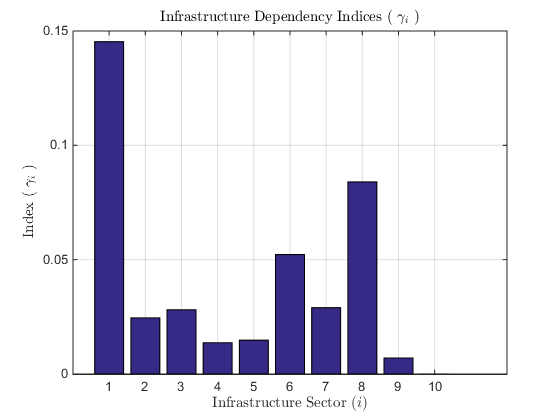
\includegraphics[width=0.8\textwidth]
    {gamma.png}
    \caption{Dependency index for all the sectors}
    \label{fig: Gamma}
\end{figure}

\begin{figure}
	\centering
	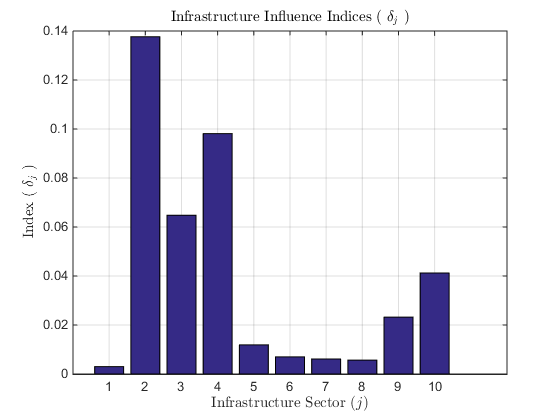
\includegraphics[width=0.8\textwidth]
    {delta.png}
    \caption{Influence index for all the sectors}
    \label{fig: Delta}
\end{figure}

From figure NUMBER, we observe that the air transportation sector (sector 1) has the highest dependency index ($\gamma_1 = 0.145$). This means that the air transportation sector
receives the biggest direct damage from the inoperability of the entire infrastructure system. The sectors of fuel and petroleum grid and rail transportation are respectively the second and third most dependent infrastructures within the system ($\gamma_8 = 0.084$  and  $\gamma_6 = 0.052$). These indices reveal that the transportation sector in general is highly dependent on other infrastructure sectors within the system and subsequently the first sector to be influenced or damaged. Other than the previous three sectors, the remaining infrastructures have low direct dependency on the inoperability of other sectors as all of the remaining indices have a value below $0.03$. Note that the satellite communication and navigation sector (sector 10) has an index of ($\gamma_10 = 0$) which indicates that sector 10 is not actually affected by the inoperability of any other infrastructure within the system.\\
\\
As for the influence index, we observe that the electricity sector (sector 2) has the highest influence index ($\delta_2 = 0.138$). This means that the electricity sector
transmits the biggest direct damage from its inoperability to the entire infrastructure system. The sectors of TLC wired and TLC wireless are respectively the second and third most influential infrastructures within the system ($\delta_4 = 0.098$  and  $\delta_3 = 0.065$). Furthermore, the satellite communication and navigation sector has a relatively high influence index ($\delta_10 = 0.041$), which reveals that inoperability of sector 10 has a sizable effect on the infrastructure system. These indices reveal that the electricity and the communication sectors in general have the largest direct impact on other infrastructure sectors as a result of their inoperability. Other than the previous four sectors, the remaining infrastructures have low direct influence on the inoperability of other sectors as all of the remaining indices have a value below $0.025$.

\subsection*{Question 10}
Similar to Question 9, the indices $\overline\gamma_i$ and $\overline\delta_j$ have been calculated using a script and a class in MATLAB.
\underline{\textbf{Note:}} For the aforementioned script and class, please refer to the appendix. For the MATLAB code, please refer to the script entitled NAME and the class entitled NAME that are uploaded on compass 2g.

The indices $\overline\gamma_i$ and $\overline\delta_j$ for every infrastructure sector are presented in the figures NUMBER AND NUMBER below.

\begin{figure}
	\centering
	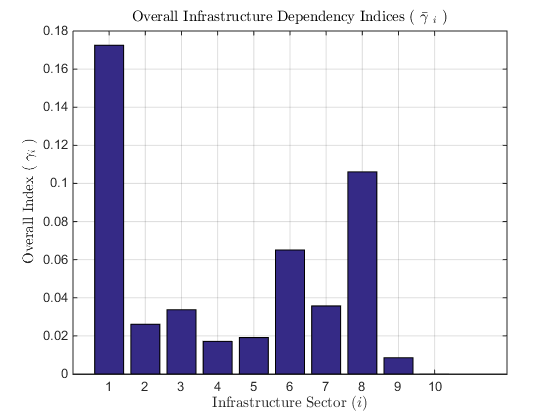
\includegraphics[width=0.8\textwidth]
    {gamma_bar.png}
    \caption{Overall dependency index for all the sectors}
    \label{fig: Gamma bar}
\end{figure}

\begin{figure}
	\centering
	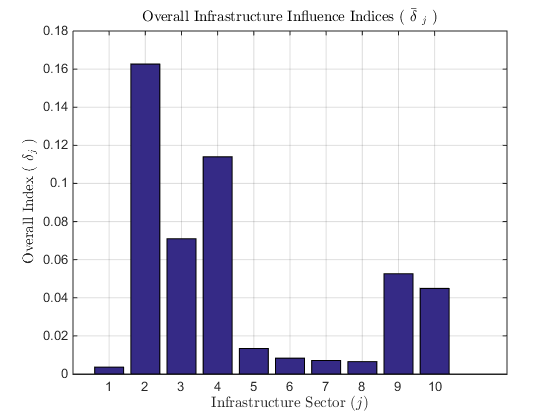
\includegraphics[width=0.8\textwidth]
    {delta_bar.png}
    \caption{Overall influence index for all the sectors}
    \label{fig: Delta bar}
\end{figure}

The comparison of the indices $\gamma_j$ and $\overline\gamma_j$ further stresses on the difference

From figure NUMBER, we observe that the air transportation sector (sector 1) has the highest dependency index ($\gamma_1 = 0.145$). This means that the air transportation sector
receives the biggest direct damage from the inoperability of the entire infrastructure system. The sectors of fuel and petroleum grid and rail transportation are respectively the second and third most dependent infrastructures within the system ($\gamma_8 = 0.084$  and  $\gamma_6 = 0.052$). These indices reveal that the transportation sector in general is highly dependent on other infrastructure sectors within the system and subsequently the first sector to be influenced or damaged. Other than the previous three sectors, the remaining infrastructures have low direct dependency on the inoperability of other sectors as all of the remaining indices have a value below $0.03$. Note that the satellite communication and navigation sector (sector 10) has an index of ($\gamma_10 = 0$) which indicates that sector 10 is not actually affected by the inoperability of any other infrastructure within the system.\\
\\
As for the influence index, we observe that the electricity sector (sector 2) has the highest influence index ($\delta_2 = 0.138$). This means that the electricity sector
transmits the biggest direct damage from its inoperability to the entire infrastructure system. The sectors of TLC wired and TLC wireless are respectively the second and third most influential infrastructures within the system ($\delta_4 = 0.098$  and  $\delta_3 = 0.065$). Furthermore, the satellite communication and navigation sector has a relatively high influence index ($\delta_10 = 0.041$), which reveals that inoperability of sector 10 has a sizable effect on the infrastructure system. These indices reveal that the electricity and the communication sectors in general have the largest direct impact on other infrastructure sectors as a result of their inoperability. Other than the previous four sectors, the remaining infrastructures have low direct influence on the inoperability of other sectors as all of the remaining indices have a value below $0.025$.

Add the S and bigger A
and then refer to upcoming questions in with the tier stuff.

Sector 10 doesn't have an increase because it is already independent.

\subsection*{Question 11}
Traditionally, an electric grid is the network  of "wires, substations, transformers, switches, and much more" that delivers electricity from the power-generating plants to the consumers (Energy.gov). On the other hand, a smart electric grid indicates that the conventional electric grid has become computerized. A grid becomes smart when "two-way digital communication and computer processing" have been introduced in the system. These incorporated technologies allow the electricity utilities to control their power generation by benefiting from better demand monitoring and management technologies (Energy.gov).\\
\\
Despite the apparent benefits of having a smart grid, such as increased efficiency, better energy security, etc... the smart technologies would modify the dependencies of the electricity sector with other sectors in the infrastructure system. To identify the changes in the dependencies in the infrastructure system, we assessed whether a 6-12 hour outage of the electricity sector would increase or decrease the propagation of inoperability on every other sector in the system. \\
\\
According to the website (WEBSITE), a smart grid will help integrate more large-scale renewable energy resources into the exisitng grid, as well as achieve a more efficient electricity generation and transmission. In our infrastructure system, a better integration of renewable energy resources translates into requiring less fossil fuels such fuel and petroleum, in addition to natural gas. This means that the electricity sector will be less influenced or dependent by the fuel and gas sector and by the natural gas sector (sectors 8 and 9), assuming that a smart grid would be fully functional. So in a 6-12 hour outage of sectors 8 and 9, the smart grid can ramp up the production of power from renewable sources in case there was no inventory of fossil fuel resources in the concerned plants.\\
\\ 
Moreover,given that a smart grid fundamentally relies on the communications sector to achieve a more efficient power generation, the electricity sector will have an increased dependency on the TLC wireless sector, TLC wired, and the satellite communication and navigation sector (sectors 3,4, and 10). So the electricity sectors will be more influenced by any damage of these aforementioned sectors.\\
\\ 
Furthermore, for the remaining sectors in the system, we considered that the dependencies with the electricity sector will not change for a 6-12 hour outage, whether this grid was either traditional or smart. For instance, the water management sector will be similarly influenced by a power outage of the electricity sector for 6-12 hours, and the electricity sector, smart or not, will be equally affected by a potential outage of the water sector for 6-12 hours.\\
\\
To sum up, the actual coefficients of matrix A that will be change are: 
\begin{itemize}
	\item Increase in the coefficients $a_{23}$, $a_{24}$ and $a_{210}$
	\item Decrease in the coefficients $a_{28}$ and $a_{29}$
	\item No change in the remaining coefficients
\end{itemize}

\subsection*{Question 12}
\begin{itemize}
	\item TODO: Matlab code to add/decrease 10%
\end{itemize}

\subsection*{Question 13}
The snow storm in this problem describes an external shock ($f$) that impacts some elements of the infrastructure system. The effect causes damage to propagate throughout the infrastructure system. The resulting damage is calculated through Equation \ref{eq: EIO Solution} with the results shown in the table below.
\begin{table}[H]
  \centering
  \caption{Damage from a snow storm}
    \begin{tabular}{r|rrrrrrrrrr}
    \toprule
    Sector Id & \multicolumn{1}{c}{1} & \multicolumn{1}{c}{2} & \multicolumn{1}{c}{3} & \multicolumn{1}{c}{4} & \multicolumn{1}{c}{5} & \multicolumn{1}{c}{6} & \multicolumn{1}{c}{7} & \multicolumn{1}{c}{8} & \multicolumn{1}{c}{9} & \multicolumn{1}{c}{10} \\
    \midrule
    Overall Damage (\%)      & 38.96 & 10.30 & 1.64 & 1.29 & 1.08 & 52.81 & 1.51 & 6.83 & 0.45 & 0 \\
    \bottomrule
    \end{tabular}%
  \label{tab: Snow storm 13}%
\end{table}%
The most damaged infrastructure was the rail transportation due to the external shock taking out 50\% of the rail network, resulting in $52.81\%$ damage to the sector. The least affected sector was the Satellite Communication and Navigation sector with no damage caused, followed by the Natural Gas sector which had $0.45\%$ damage.
Additional damage done to the air transportation sector, electricity sector, and rail transportation sector due to the propagation of damage through the infrastructure system resulted in further degradation of $3.96\%$ for air transportation, $0.30\%$ for electricity, and $2.81\%$ for rail transportation. When only considering the damage propagated throughout the system, the most damaged infrastructure would be the fuel and petroleum grid at $6.83\%$ degradation. The least damaged system does not change from the satellite communication and navigation sector but the second least damaged infrastructure would be the electricity sector at $0.30\%$ rather than the natural gas sector at $0.45\%$.

\subsection*{Question 14}
Matrix $A$ is not an appropriate influence matrix to analyze the effects of a heavy snow storm. This is because matrix $A$ contains many limitations inherent within the matrix itself.\\
\\
One of the limitations within the matrix $A$ is that the values in the matrix are for an outage of 6-12 hours and there is no guarantee that the snow storm will last within that time range. Though in the Setola et. al paper, there were additional matrices to account for the different lengths of outages; the matrix $A$ given does not account for these differences\\
\\
Another limitation of matrix $A$ consist of how the data to create the values in the matrix were collected. The information was gathered through questionnaires given to experts within each sector asking about how an outage of another sector would influence the operability of their sector (Setola, 2009). There are no means to know the number of experts that were questioned and to objectively assess each answer since every response to the questionnaire was subjective and was given one value ranging from 0 to 0.5 depending on the response of the expert. There is also the inherent assumption that the experts know the direct influence each of the other sectors has on their sector.\\
\\
Though the matrix $A$ attempts to account for uncertainty from the answers to the questionnaire using fuzzy numbers, each expert had no idea on how their answers would be translated to a numerical value. Furthermore, the fuzzy numbers that was used to capture the uncertainty within the answers consisted of additional uncertainties about the reliability of the expert, and the confidence level of the expert which again assigns values to subjective answers ($+/-0.005$ to $+/-0.02$) (Setola, 2009).

\subsection*{Question 15}
Question 4 presented the analytical solution $x=Sf$ for the overall propagation of damage of the infrastructure system. This solution was obtained using properties of linear algebra. \\
\\
This solution can be supported by studying the step-by-step propagation of damage of an infrastructure system. The damage propagation starts from zero-damage state, continues by absorbing the external impact $f$, and recursively computes additional damage derived from the preceding step (the additional damage from the previous damage). After a number of damage propagation steps, the state of the system should match that found using the equation presented in Question 4. \\
\\
A recursive function was implemented in MATLAB for this purpose. The source code can be found in the Appendix and in the attached files, along with the documentation that gives instructions for running it. Figure \ref{fig: Damage Propagation 1-10} presents 10 tiers of damage propagation, starting from the $0_{th}$ tier (initial conditions with no damage) to the $10_{th}$ tier. Similarly, Figure \ref{fig: Incremental Damage Propagation 1-10} presents the incremental damage on each sector after each damage propagation step. \\
\\
Note that the damage propagation steps presented in Figure \ref{fig: Damage Propagation 1-10} converge to the same values found in Question 13 after a $k$ number of steps. This is further explained by the damage increments after a certain number of propagation steps approaching zero, as seen in Figure \ref{fig: Incremental Damage Propagation 1-10}. The system damage at $k=0$ is zero, but approaches to the solution from $x=Sf$ after a number of tiers, which may vary from sector to sector. That is, some sectors may converge to faster than others. Initially the damage increments are generally large, but approach zero after the solution from $x=Sf$ is approached. This is not a coincidence, it is purely a property of linear algebra: $(I-A)^{-1}f=Sf$ is the damage propagation at an infinite number of propagation steps. 
\begin{figure}[H]
	\centering
	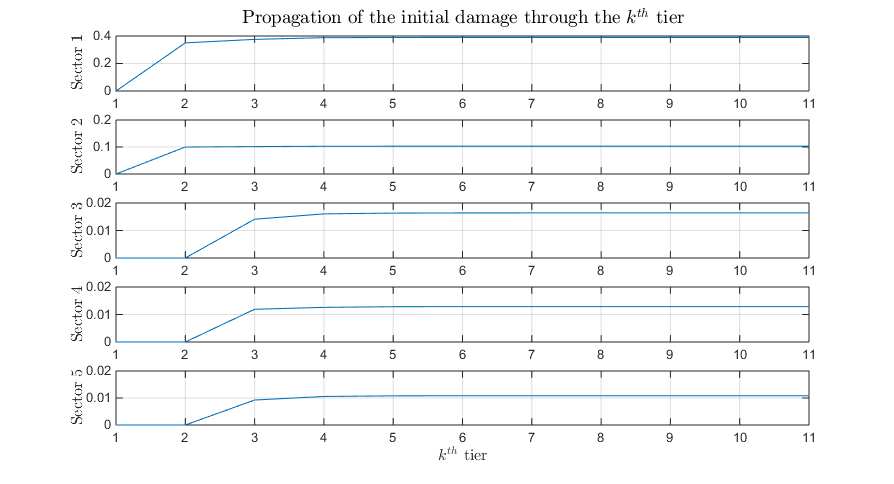
\includegraphics[width=1\textwidth]
    {damage_propagation_1_5.png}
	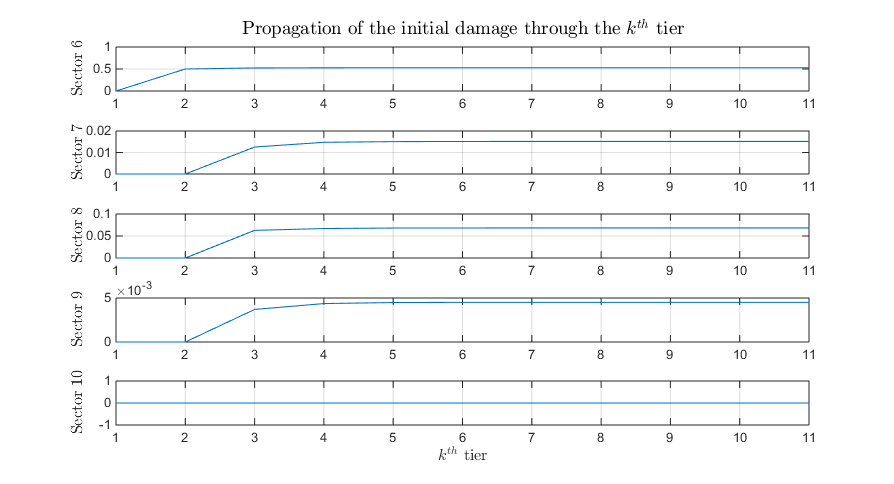
\includegraphics[width=1\textwidth]
    {damage_propagation_6_10.png}
    \caption{Ten tiers of damage propagation for sectors 1 through 10.}
    \label{fig: Damage Propagation 1-10}
\end{figure}

\begin{figure}[H]
	\centering
	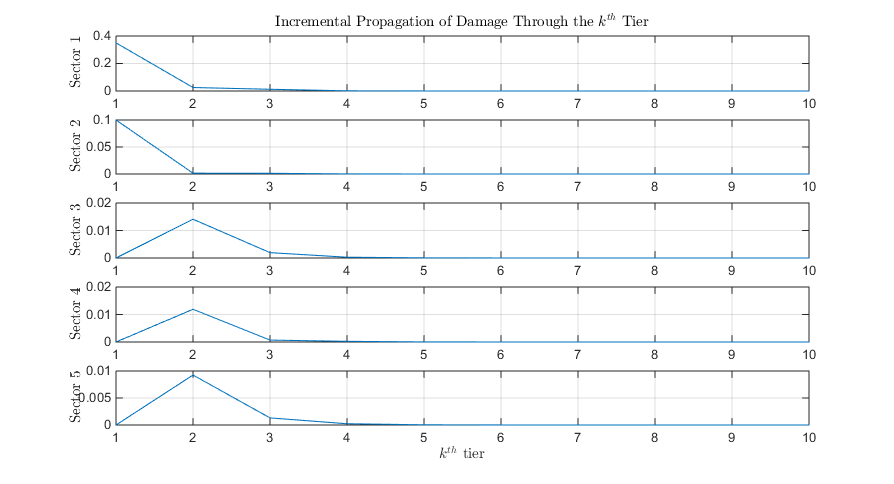
\includegraphics[width=1\textwidth]
    {incremental_damage_propagation_1_5.png}
	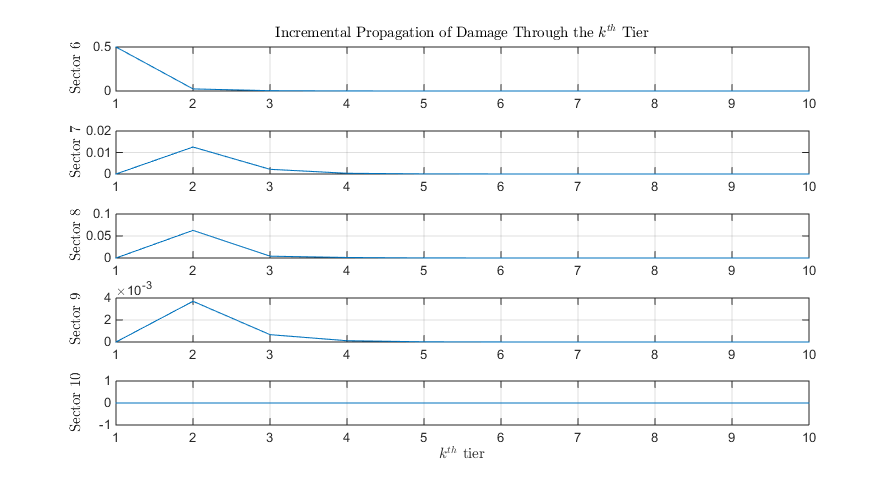
\includegraphics[width=1\textwidth]
    {incremental_damage_propagation_6_10.png}
    \caption{Ten tiers of incremental damage propagation for sectors 1 through 10.}
    \label{fig: Incremental Damage Propagation 1-10}
\end{figure}

\subsection*{Question 16}
One thousand replications of Monte Carlo simulation were performed for modeling uncertainty in matrix $A$. Specifically, noise was added to the elements of matrix $A$ using a uniform distribution that ranged from $-15\%$ to $-15\%$ of each value. That is, each element $a_{ij}$ of matrix $A$ was updated using
\begin{align}
	a_{ij} = a_{ij} \cdot (100\% - 15\%) + U(0,1) \cdot a_{ij} \cdot (30 \%).
	\label{eq: Noise}
\end{align} 
The results of the simulation can be found as histograms of $100$ bins in Figure \ref{fig: Histograms Monte Carlo A}. Important statistical descriptors can be found in Figure \ref{fig: Box Plots Monte Carlo A} as box plots. \\
\\
\begin{figure}
	\centering
	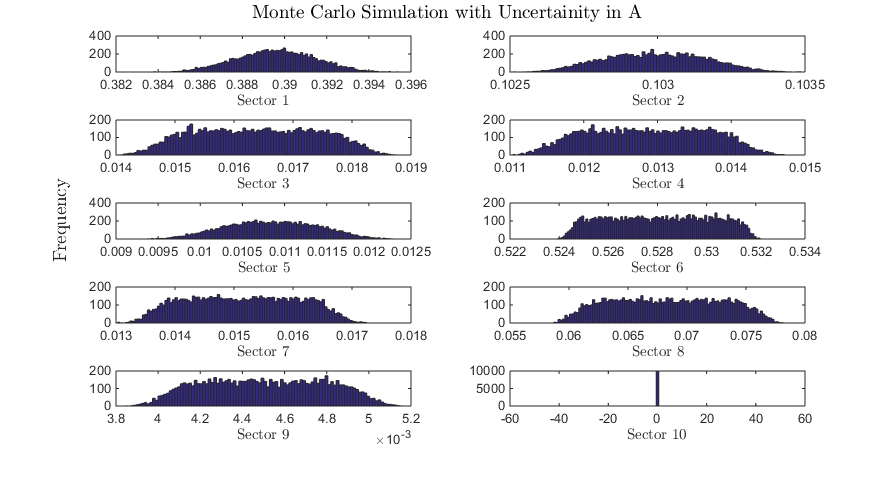
\includegraphics[width=1\textwidth, height=10cm]
    {monte_carlo_A_1000_100.png}
    \caption{Histograms of Monte Carlo simulation on overall damage propagation for each sector with uncertainty in $A$.}
    \label{fig: Histograms Monte Carlo A}
\end{figure}
\begin{figure}
	\centering
	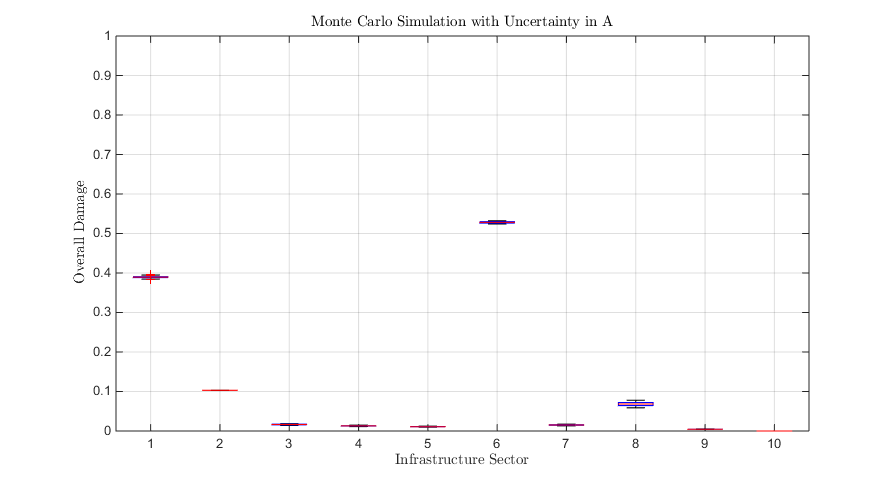
\includegraphics[width=1\textwidth]
    {monte_carlo_A_1000_100_box_plot.png}
    \caption{Box plots of Monte Carlo simulation on overall damage propagation for each sector with uncertainty in $A$.}
    \label{fig: Box Plots Monte Carlo A}
\end{figure}
From Figure \ref{fig: Box Plots Monte Carlo A} we observe that it is not trivial to determine whether the overall damage propagation follows a uniform distribution, a normal distribution, or some other distribution. This is expected, as the influence of the uncertainty in each sector may influence a given sector may vary. 

\subsection*{Question 17}
One thousand replications of Monte Carlo simulation were performed for modeling uncertainty in vector $f$. Specifically, noise was added to the elements of matrix $f$ using a uniform distribution that ranged from $-15\%$ to $-15\%$ of each value using Equation \ref{eq: Noise}. \\
\\ 
The results of the simulation can be found as histograms (of $100$ bins) in Figure \ref{fig: Histograms Monte Carlo f} and box plots in Figure \ref{fig: Box Plots Monte Carlo f}.
\begin{figure}[H]
	\centering
	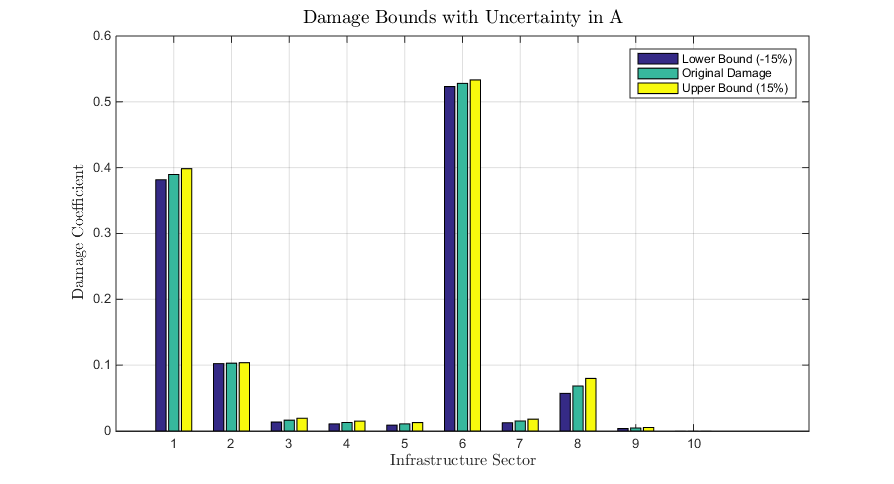
\includegraphics[width=1\textwidth, height=10cm]
    {damage_bounds_uncertainty_A.png}
    \caption{Bounds on overall system damage with a $-15\%$ to $15\%$ uniformly distributed uncertainty in $A$.}
    \label{fig: Damage Bounds A}
\end{figure}
\begin{figure}[H]
	\centering
	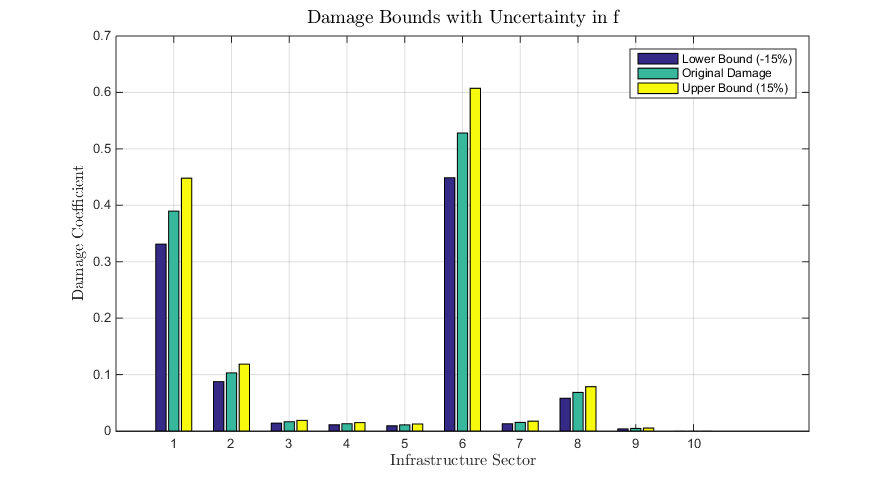
\includegraphics[width=1\textwidth]
    {damage_bounds_uncertainty_f.png}
    \caption{Bounds on overall system damage with a $-15\%$ to $15\%$ uniformly distributed uncertainty in $f$.}
    \label{fig: Damage Bounds f}
\end{figure}


\subsection*{Question 18}
\begin{figure}
	\centering
	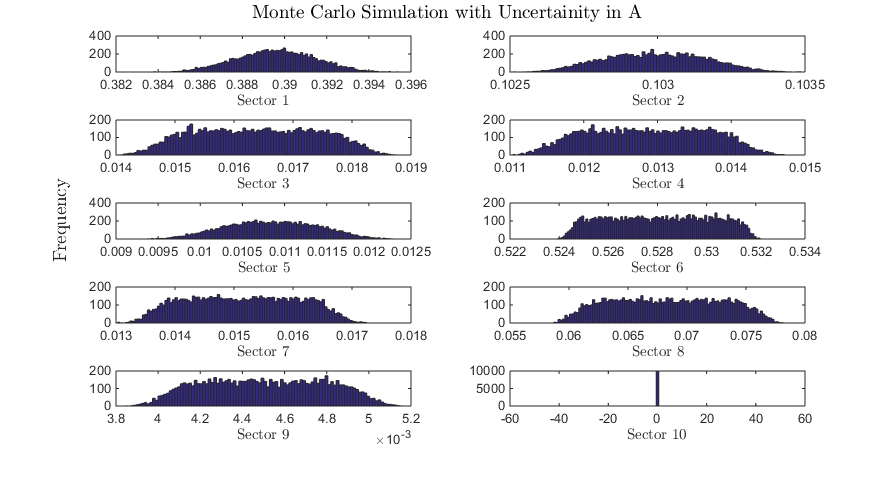
\includegraphics[width=1\textwidth, height=10cm]
    {monte_carlo_A_1000_100.png}
    \caption{Histograms of Monte Carlo simulation on overall damage propagation for each sector with uncertainty in $A$.}
    \label{fig: Histograms Monte Carlo A}
\end{figure}
\begin{figure}
	\centering
	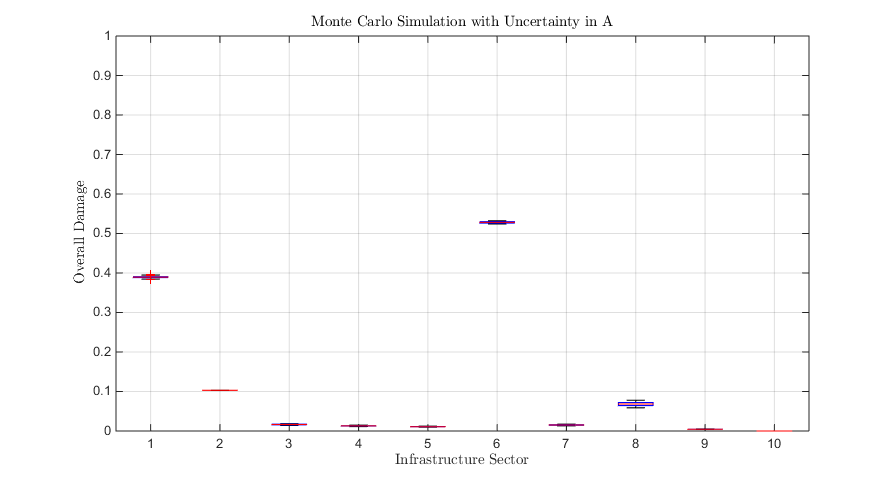
\includegraphics[width=1\textwidth]
    {monte_carlo_A_1000_100_box_plot.png}
    \caption{Box plots of Monte Carlo simulation on overall damage propagation for each sector with uncertainty in $A$.}
    \label{fig: Box Plots Monte Carlo A}
\end{figure}

\subsection*{Question 19}

\section*{Electricity Utilities}
\subsection*{Question 20}
There are three sets that compose the decision variables, which are:
\begin{align*}
	& x_{it},  \forall  i \in \{1,2,3,4,5,6,7,8,9\}, \forall  t \in \{1,2,3,4,5,6\}\\
	& y_i,  \forall  i \in \{5,6,7,8\}\\
	& z_k,  \forall  k \in \{1,2,3\}
\end{align*}
where $x_{it}$ is the energy (MW) produced by power plant $i$ during load block $t$,
$y_i$ is the design capacity of new power plant $i$ (MW), and $z_k$ is the implementation rate of demand side management program $k$, such that $z_k \in  [0,1]$. This amounts to 61 decision variables. 
\begin{itemize}
	\item The decision variable vector NAMELESS will be a column vector with dimensions 61 x 1. OR the decision variable vector lives in the space of $R^{61}$
\end{itemize}

\subsection*{Question 21}
The expression for the objective function which minimizes the total global warming potential is:
\begin{align*}
	\min \sum_{i=1}^{9}\sum_{t=1}^{6} g_{i}x_{it}n_{t}
\end{align*}
where $g_{i}$ is the global potential (kg $CO_2$ eq/MWh) from plant $i$, and $n_{t}$ is the number of hours in load block $t$ (MW).\\
Note that this expression will result in the minimum global warming potential in the units of kg of $CO_2$ eq, instead of tons of $CO_2$ eq. The unit conversion does not affect the solution from the optimization problem. We will convert the units of the solution accordingly.

\subsection*{Question 22}
The expression for the objective function which minimizes the expected annual cost of operating the utility is:
\begin{align*}
	\min \sum_{i=1}^{9}\sum_{t=1}^{6} \bar{c_{i}}^{v}x_{it}n_{t} + \sum_{i=5}^{8}\bar{c_{i}}^{c}y_{i}\cdot 10^3 + \sum_{k=1}^{3}\sum_{t=1}^{6}\bar{c_{k}}^{d}z_{k}s_{kt} ^{\text{\textit{max}}}n_{t}
\end{align*}
where,
\begin{itemize}
	\item $\bar{c_{i}}^{v}$ is the expected variable cost associated with operating plant $i$ (\$/MWh)
	\item $\bar{c_{i}}^{c}$	is the expected annualized capital cost of  plant $i$ (\$/kW). Note that we multiplied the values of the design capacities of new power plants, $y_i$ by a factor of $10^3$ to convert the units from MW to kW
	\item $\bar{c_{k}}^{d}$ is the expected cost of implementing demand side management program $k$ (\$/MWh)
	\item $s_{kt} ^{max}$ is the maximum energy savings available in load block $t$ from demand side management program $k$ (MW)
\end{itemize}

\subsection*{Question 23}
The written expression for the load constraints for the power plants is:
\begin{align*}
	\sum_{i=1}^{9}x_{it} + \sum_{k=1}^{3}z_{k}s_{kt}^{\text{\textit{max}}}\geq l_{t},   \forall t\in{}\{1,2,3,4,5,6\}\\
\end{align*}
where $l_{t}$ is the power load in load block $t$ (MW). This constraint forces the electricity utilities to produce at least the required power needed for each load block. Since this constraint applies to each load block, there are six constraints in total.

\subsection*{Question 24}
The expression for the instantaneous capacity constraints of the power plants is:
\begin{align*}
	x_{it} \leq (1 - o_{i}^{u})x_{i}^{\text{\textit{max}}},	\forall i \in{} \{1,2,3,4,5,6,7,8,9\}, \forall t\in{}\{1,2,3,4,5,6\}\\
\end{align*}
where $o_{i}^{u}$ is the unplanned outage rate with values ($\in{} [0,1]$). 
CHECK THESE STATEMENTS!!! (see which one we should keep)
\begin{itemize}
	\item This constraint determines the time during which the plant is operational, adjusting the maximum capacity of the plant accordingly and thus forcing the energy produced to never exceed this capacity.
	\item This is an attempt to account for the periods of time where there is no power coming from a power plant $i$ due to an unexpected outage 
\end{itemize}
This constraint applies to every decision variable $x_{it}$ so there are fifty-four constraints.

\subsection*{Question 25}
The expression for the minimum generation constraints is given by:
\begin{align*}
	x_{it} \geq x_{i}^{\text{\textit{min}}},	\forall i \in{} \{1,2,3,4,5,6,7,8,9\}, \forall t\in{}\{1,2,3,4,5,6\}\\
\end{align*}
where $x_{i}^{min}$ is the minimum capacity of the power plant. This constraint makes it so that the energy produced in power plant $i$ is never less than the minimum amount of power that the plant needs to generate. This constraint holds true for all power plants and during all load blocks ($\forall i \in{} \{1,2,3,4,5,6,7,8,9\},  \forall t \in{} \{1,2,3,4,5,6\}$), therefore there are fifty-four constraints.

\subsection*{Question 26}
New generation bounds is similar to the instantaneous capacity constraints except for the power plants that are newly built. Basically, the energy produced in power plant $i$ during load block $t$ must be less than or equal to the the derated capacity for each plant caused by unplanned outages: $(1-o_{i}^{u})y_{i}$, where $y_{i}$ is the design capacity of power plant $i$ (MW)($\forall i \in{} \{5,6,7,8\},  \forall t \in{} \{1,2,3,4,5,6\}$)\\
\\
Additionally, the new generation bounds make sure that the design capacity of the power plant is less than or equal to the maximum capacity that can be built with the following expression:
\begin{align*}
	y_{i} \leq x_{i}^{\text{\textit{max}}}, \forall i \in{} \{5,6,7,8\}
\end{align*}

\subsection*{Question 27}
The complete optimization problem for minimizing expected costs subject to the production constraints is:
\begin{align*}
	\min & \sum_{i=1}^{9}\sum_{t=1}^{6} \bar{c_{i}}^{v}x_{it}n_{t} + \sum_{i=5}^{8}\bar{c_{i}}^{c}y_{i}\cdot 10^3 + \sum_{k=1}^{3}\sum_{t=1}^{6}\bar{c_{k}}^{d}z_{k}s_{kt} ^{\text{\textit{max}}}n_{t}\\
	s.t. & \\
	& \sum_{i=1}^{9}x_{it} + \sum_{k=1}^{3}z_{k}s_{kt}^{\text{\textit{max}}}\geq l_{t},   \forall t\in{}\{1,2,3,4,5,6\}\\
	& x_{it} \leq (1 - o_{i}^{u})x_{i}^{\text{\textit{max}}},	\forall i \in{} \{1,2,3,4,5,6,7,8,9\}, \forall t\in{}\{1,2,3,4,5,6\}\\
	& \sum_{t=1}^{6}n_{t}x_{it} - (1 - o_{i}^{p})8766x_{i}^{\text{\textit{max}}} \leq 0, \forall i \in{} \{1,2,3,4,9\}\\
	& \sum_{t=1}^{6}n_{t}x_{it} - (1 - o_{i}^{p})8766y_{i} \leq 0, \forall i \in{} \{5,6,7,8\}\\
	& x_{it} \geq x_{i}^{\text{\textit{min}}},	\forall i \in{} \{1,2,3,4,5,6,7,8,9\}, \forall t\in{}\{1,2,3,4,5,6\}\\
	& z_{k} \geq 0, \forall k \in{} \{1,2,3\}\\
	& z_{k} \leq 1, \forall k \in{} \{1,2,3\}\\
	& x_{it} \leq (1 - o_{i}^{u})y_{i},	\forall i \in{} \{5,6,7,8\}, \forall t\in{}\{1,2,3,4,5,6\}\\
	& y_{i} \leq x_{i}^{\text{\textit{max}}}, \forall i \in{} \{5,6,7,8\}\\
\end{align*}
There are one hundred and fifty-seven constraints in this problem.\\
The constraints are split into the following categories:
\begin{itemize}
	\item Six are from the load constraints
	\item Fifty-four are from the instantaneous capacity constraints
	\item Five are from the annual energy constraints of the existing plants
	\item Four are from the annual energy constraints of the new plants
	\item Fifty-four are from the minimum generation constraints
	\item Six are the bounds on the DSM programs
	\item Twenty-eight constraints are for the new generation bounds.
\end{itemize}
\subsection*{Question 28}

\subsection*{Question 29}

\subsection*{Question 30}

\subsection*{Question 31}

\subsection*{Question 32}

\subsection*{Question 33}

\subsection*{Question 34}

\subsection*{Question 35}

\subsection*{Question 36}

\subsection*{Question 37}


\end{document} 